%-------------------------------------------------------------------------------------------------------
%-------------------------------------------------------------------------------------------------------
\chapter{The LCS Runtime Library RtLib}

Intended for the node firmware programmer, the LCS runtime library is the main interface to the hardware module. The library has methods for node and port configuration, event processing and layout control bus management. Most of the LCS bus management, node, port and port data management is performed transparently to the node firmware programmer. The library also provides convenience methods to send messages to other nodes and allows for a rich set of callback functions to be registered to act on messages and events.

The key design objective for the runtime library is to relief the LCS nodes firmware programmer as much as possible from the details of running a firmware inside a hardware module. Rather than implementing the lower layers for storage and message processing at the firmware level, the runtime library will handle most of this processing transparently to the upper firmware layer. A small set of intuitive to use and easy to remember functions make up the core library. The library communicates back to the firmware layer via a set of defined callbacks. Throughout the next chapters, the library will be presented in considerable detail. Let's start with the high level view.

The following figure depicts the overall structure of a LCS hardware module and node. At the bottom is the hardware module, which contains the communication interfaces, the controller and the node specific functions. The core library offers a set of APIs and callbacks to the node firmware. The firmware programmer can perform functions such as sending a message or accessing a node attribute through the APIs provided. The library in turn communicates with the firmware solely via registered callbacks.

picture 

\begin{figure}[h]
    \centering
   % 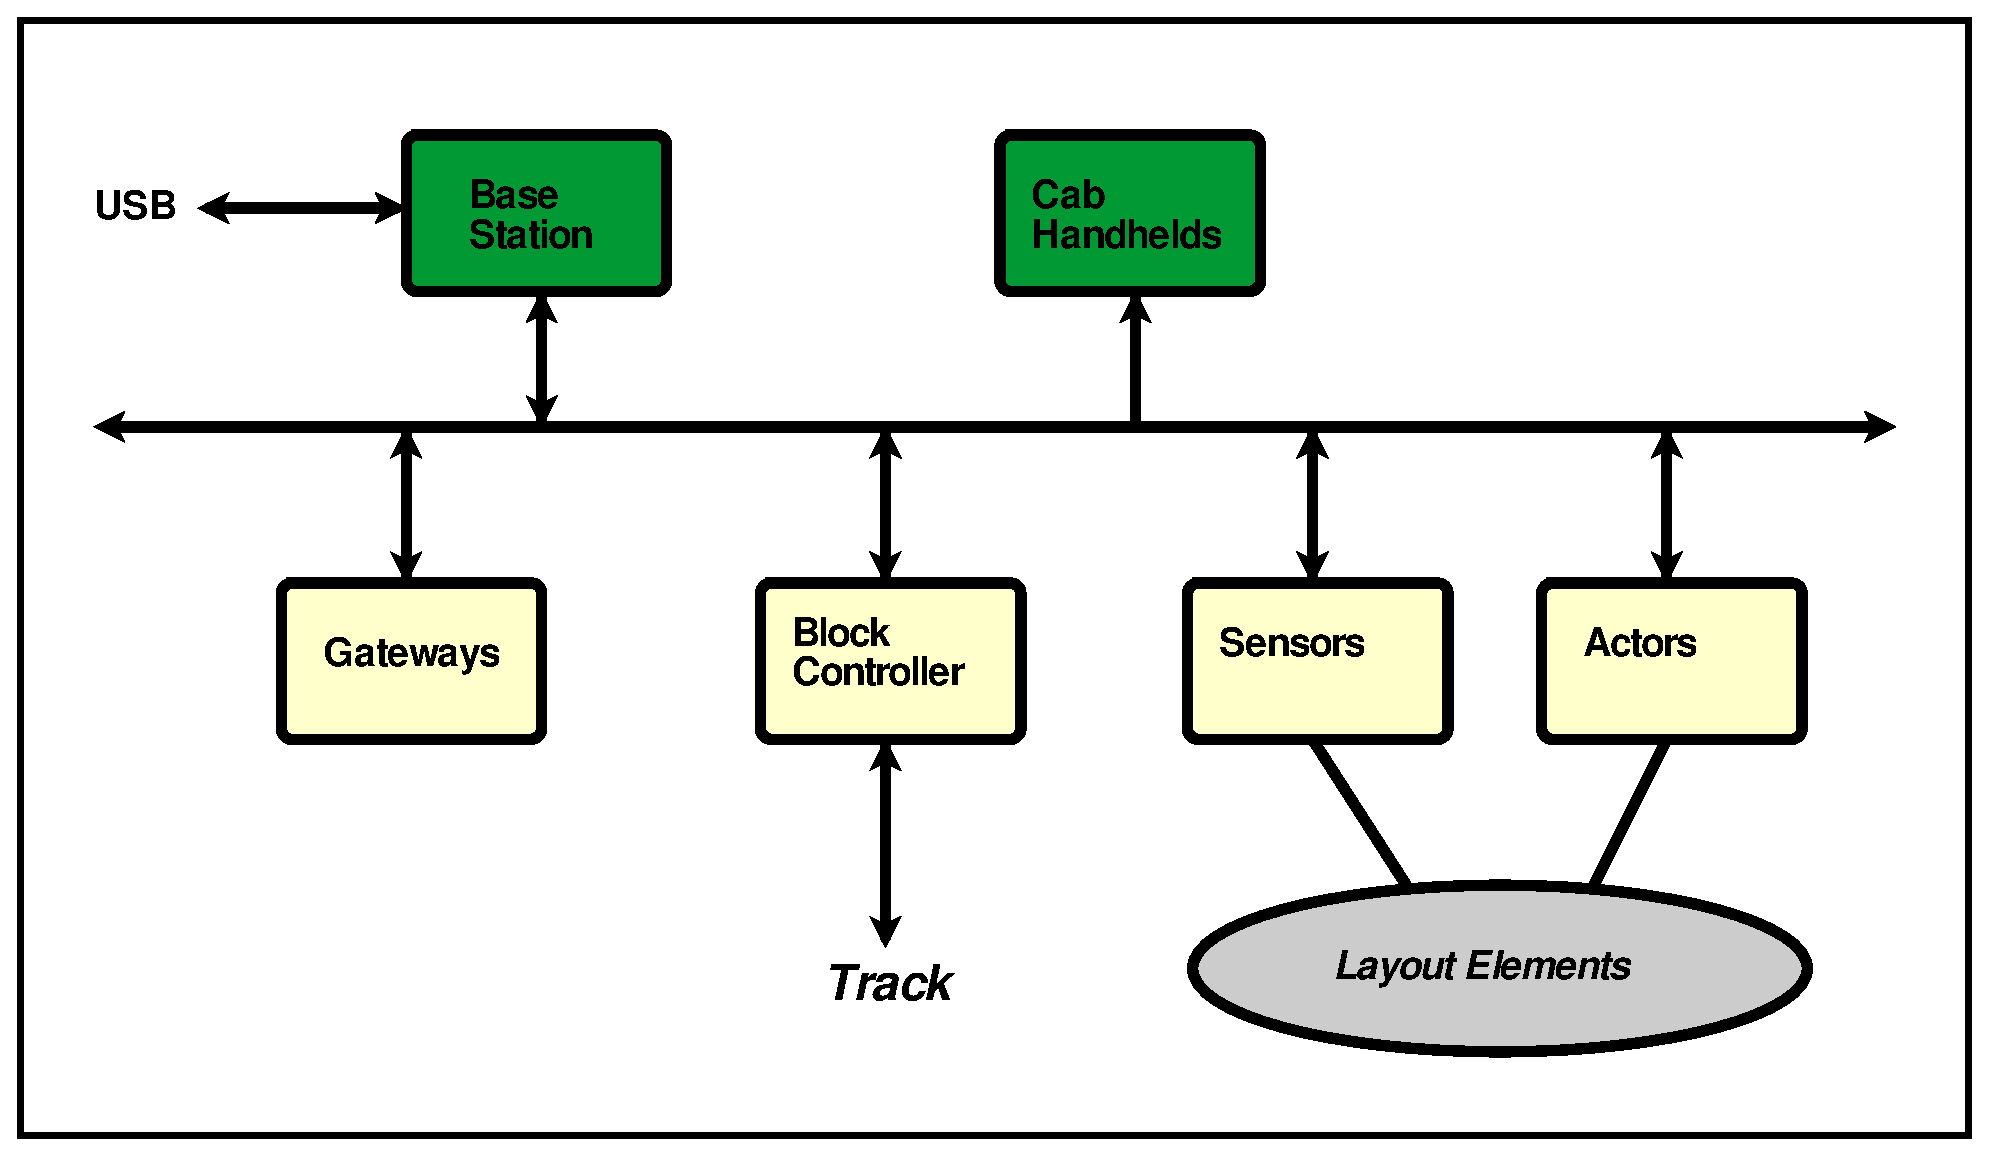
\includegraphics[page=1, width=\textwidth]{./figures/Schematic_LcsNodes-Layout-Overview.pdf}
   %![Schematic_LcsNodes-Core-Library-Overview.png](./Figures/Schematic_LcsNodes-Core-Library-Overview.png )
\end{figure}

The firmware has of course also direct access to the hardware module capabilities. This is however outside the scope for the LCS core library. As we will see in the coming chapters, the library has a rich set of functions and does also perform many actions resulting form the protocol implementation transparently to the firmware programmer. It is one of the key ideas, that the firmware programmer can concentrate on the module design and not so much on the inner workings of the LCS layout system. Events, ports, nodes and attributes form a higher level foundation for writing LCS control system firmware. Not all of the functionality will of course be used by every node. A base station and a handheld cab control will for example make heavy use of the DCC commands. A turnout device node will use much more of the port and event system. Size and functions of the various library components can be configured for a node.

As a consequence, the library is not exactly a small veneer on top of the hardware and does take its program memory toll on controller storage. However, with the growing capabilities of modern controllers, this should not be a great limitation. The first working versions required an Arduino Atmega1284 alike version as the controller. The current working version is based on the Raspberry Pi Pico controller. More on the individual requirements and selection later.

The appendix contains the detailed description of all library interfaces. If a picture says more than a thousands words, an excerpt of the data declarations from the implementation says even more to the firmware programmer. At the risk of some minor differences on what is shown in the book and the actual firmware, you will find a lot of declarations directly taken from the "LcsRuntimeLib.h" include file.

%-------------------------------------------------------------------------------------------------------
%-------------------------------------------------------------------------------------------------------
\chapter{RtLib Storage}

All data of a LCS node is kept in volatile \texttt{(MEM)} and non-volatile \texttt{(NVM)}. The data is structured into several data areas which we call **map**s. A map is a memory area which can be found in MEM and NVM or only in MEM. The key idea is that a map in MEM is initialized from its NVM counterpart at runtime start. Changes in a MEM map can be synced with its NVM map counterpart. There are also maps that do not have a NVM counterpart. These maps are initialized with default values defined for this map. 

Maps do of course have a size. A port map for example will have a number of entries, one for each port. The design choice was whether all map sizes are configurable or rather a fixed size. The current design features a fixed size scheme. There are a few key reasons for this decision. First, there is no configuration need when initializing a node. Second, the total size even when generously sizing the maps is rather small compared to what the hardware can do. A node with 64 node attribute, 15 ports each of which also have 64 port attributes, an event map of 1024 events to manage and space for some miscellaneous date items will be around 8 Kbytes of data. A node with a 32K NVM chip still has plenty of space for user data. A raspberry Pi PICO has 264Kbytes of MEM, so also not an issue. Finally, with a fixed map layout, the NVM data can be copied in one swoop to a memory area on runtime start or reset. 

This chapter presents a high level overview of the available maps and their purpose. Instead of painting many pictures, we will directly take code snippets from the runtime include files to show the data found in each map. Note that all maps are only accessible via runtime library routines.

\section{Node Map}

The node map is a node private data structure only accessible to the library firmware. It contains the information about the configured maps, the node options, nodeId, canId and other data such as the library version. When a node is initially created the configuration descriptor contains all the required information to set up a node map. Nodes need volatile and non-volatile storage. Our design implements a mirroring scheme. For the LCS storage there is a memory and an EEPROM version with the same layout. When a node is running the memory version is the storage to use for performance reasons. Also, it can be expected that the memory contents changes very often during operation. EEPROMs do have a limited number of writes in their lifetime and are not that performant for a write cycle. On the other the other hand the data is stored non-volatile. Information that needs to be changed and available across a restart is therefore synced from MEM to NVM. On restart, the NVM data is just copied to MEM. We always start with a defined state. The following figure shows the nodeMap data structure.


picture: the high level structure of the node map...

\begin{figure}[h]
    \centering
   % 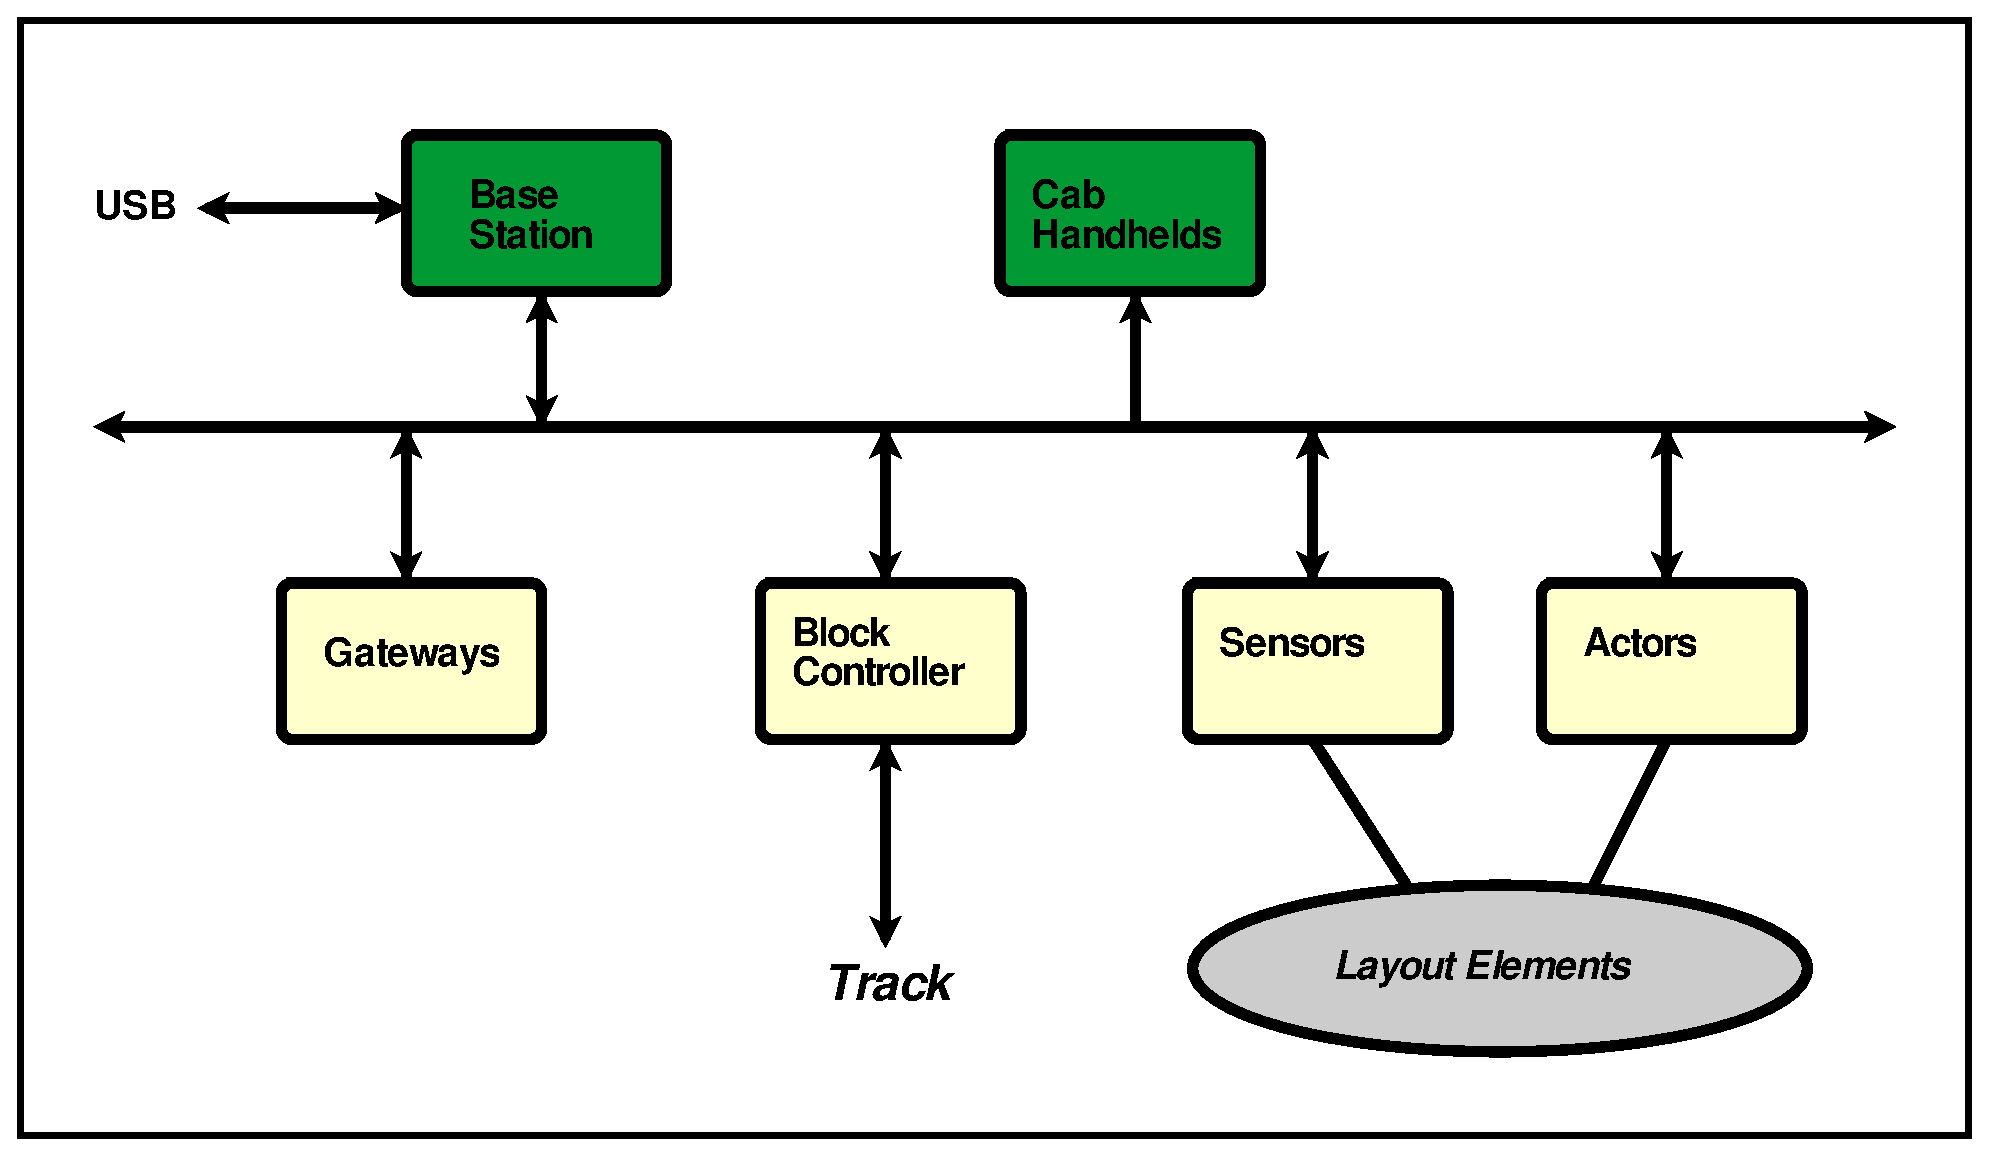
\includegraphics[page=1, width=\textwidth]{./figures/Schematic_LcsNodes-Layout-Overview.pdf}
   %![Schematic_LcsNodes-Core-Library-Overview.png](./Figures/Schematic_LcsNodes-Core-Library-Overview.png )
\end{figure}

Most of the data items deal with the location and entry sizes of the key maps. In addition, there are the nodeId, the node name, creation options, actual status flags and the set of node map attributes. Finally, the software version of the node version is kept here. For the firmware programmer there are methods to read from and write an item to the node. The library the \textbf{nodeGet}, \textbf{nodePut} and \textbf{nodeReq} routines offer a controlled access to the node map and other node data for node firmware programmers. They both use an item / value concept. Each routine passed an item Id for the data of interest and the data value. We will see an example later in this chapter. There are also three LCS messages, \texttt{(QRY-NODE)}, \texttt{(REP-NODE)} and \texttt{(SET-NODE)} which allow for access from another node. Since these messages come from another node, there is also the option to register a callback for access control checks to node data before the operation is performed.

\section{Port Map}

The port map is an array of port map entries. The maximum number of ports are set through the node configuration descriptor values set by the firmware programmer. Changing the number of ports results in a node re-initialization, rebuilding the port map and all non-volatile port map data lost. During runtime there is a non-volatile and a memory version of this map. On node startup or reset, the non volatile port map entries are copied to their memory counterpart.

\lstset{language=c++, style=codesnippetstyle}
\begin{lstlisting}
struct LcsPortMapEntry {

  
};
\end{lstlisting}

The port map entry contains flags that describe the port configuration options and the current operational setting. The event handling fields hold for an inbound port the current event received, the action and value as well as the a possible time delay before invoking the callback. For an outbound port the event fields describe the event to send when the condition for sending that event is encountered. The port map entries are located by just indexing into the port map.

The library \textbf{nodeGet}, \textbf{nodePut} and \textbf{nodeReq} routines presented before, offer a controlled access to the port map entry. The item and portId passed determine whether a node or port item is requested. Depending on the item, a portId of 0 will refer to all ports on the node or the node itself.

\section{Node and Port Items}

The term "item" came up numerous times by now. Nodes and ports features to access their attributes through an \textbf{item Id}. An item Id is just a number in the range from 1 to 255. Here is the definition from the library include file. The include file also contains the item numbers for the reserved node info and control items.

\begin{table}[h!]
    \begin{center}
        \caption{Item ranges}
        \begin{tabular}{|l|l|p{0.72\textwidth}|}
            \toprule
            \textbf{Low} & \textbf{High} & \textbf{Purpose} \\
            \midrule
            0 & & NIL Item \\
            \midrule
            1 & 63 & Reserved items for node and ports \\
            \midrule
            64 & 127 & user defined items passed to the registered callback function \\
            \midrule
            128 & 191 & Node or Port Attributes first copied from NVM to MEM and then returned \\
            \midrule
            192 & 255 & Node or Port Attributes first copied from NVM to MEM and then returned \\
            \bottomrule
        \end{tabular}
    \end{center}
\end{table}

The first set of item numbers are reserved by the core library itself for node and port items that are standardized across all nodes. The range 64 to 127 and 128 to 191 describes the set of node or port attributes. The two groups actually represent the same attributes. For example the item number 64 refers to the same attributes as item 128 does. The difference is that the latter group also accesses the NVM storage. Items 192 to 255 are completely user defined. Using these numbers will just result in a callback invocation. Note that a callback can do anything. For example, turning a signal on or off could be an item Id of let's say 205 and sending a node control message with the item 205 and the value of 1 in the first argument would result in invoking a callback which implements how to turn the signal on. In short, a node supports variable access, comparable to the CV concept in DCC, and also a function call concept which allows a great flexibility for the firmware programmer.

\section{Event Map}

The event map is an array of event map entries, each containing the eventId that node is interested in and the port Id to inform when the event is encountered. The maximum number of event map entries is set through the node configuration descriptor values set by the firmware programmer. When a new node is configured, this value is used to construct the empty event map. Any change of this value results in a node re-initialization of the node, rebuilding the event map with all non-volatile event map data lost.

\lstset{language=c++, style=codesnippetstyle}
\begin{lstlisting}
struct LcsEventMapEntry {

    uint16_t	eventId;
    uint16_t 	portId;
};
\end{lstlisting}

??? explain the SYNC approach for this map...

Like all other maps, the event map is stored in two places. The non-volatile version of the eventMap is an array of event map entries. Whenever a new entry is added, a free entry is used to store this information. The memory version of the event map is a sorted version of all used non-volatile entries. The entries are first sorted by event Id. For entries with the same event Id, the port Id is then sorted in ascending order.

In addition to the search function, event map entries can be added and deleted by specifying the eventId and portId. EventMap entries can also be accessed by their position in the event map. This is necessary to read out the event map for example though a configuration tool. While reading an event map entry from the event map is supported in both node configuration and operation mode, deleting or adding an entry is only supported in node configuration mode.

\section{User defined maps}

In addition to the runtime maps for node, ports, and events, the LCS runtime offers a user map for the firmware to use. This storage area is simply an unstructured array and the size depends on the capability of the node hardware NVM storage size. The area is the remaining storage available in the NVM chip array.

 ??? explain the concept and purpose ...

 \section{Periodic task Map}

\lstset{language=c++, style=codesnippetstyle}
\begin{lstlisting}

    User map \dots

\end{lstlisting}

 \section{Pending Request Map}

The pending request map, is a small map that keeps track of outstanding reply messages to a previously issued message request. If a node sends a request, an entry is added to this map that indicates that a reply from another node is pending. When a reply messages is detected, the firmware callback is only invoked if this reply matches a previous request. This map is a volatile structure, a restart will clear all outstanding requests.

??? a timeout concept

\section{Driver function map}

\lstset{language=c++, style=codesnippetstyle}
\begin{lstlisting}

... code snippet here ...

\end{lstlisting}

\section{Driver map}

for extension boards to be explained later...

\lstset{language=c++, style=codesnippetstyle}
\begin{lstlisting}

... code snippet here ...

\end{lstlisting}

\section{Summary}

??? explain again why this NVM is key and thus important...

To summarize, node storage is organized in maps. 

There is the node map, which is the global place for locating all other areas in the node. The port map contains the data for the configured ports. The event map is the mapping mechanism for events to ports. During node startup, the non-volatile data is copied to a newly allocated memory area. After initialization the node will only work from the memory area. All read and write operations use the memory storage area. When setting a value in any map, the flush option allows for setting its non-volatile counter part as well, so that we have a new initial value for the next restart.

Any change to the structure of the maps, for example changing the number of entries in a map, but also a different size of a data structure caused by a new library version, will result in a rebuilding of the non-volatile memory area with all previous data lost. The layout configuration data, such as the mapping of events to the node and port needs to be stored for example in a computer system so that can be reloaded once a node is re-created. A node has no way of keeping stored data across structural changes to its map layout.

%-------------------------------------------------------------------------------------------------------
%-------------------------------------------------------------------------------------------------------
\chapter{RtLib Call Interface}

??? this chapter needs to be reworked for new library call interface....

The LCS runtime library is the foundation for any module firmware written. The library presents to the firmware programer a set of routines to configure, manage the LCS node and use the LCS functions, such as sending a message. This chapter will present the key functions used. We will look at library initialization, obtaining node information, controlling a node aspect, reacting to an event and sending message to other nodes.
Refer to the appendix for a complete set of available LCS runtime functions.

\section{Library initialization}

The LCS runtime is initialized with the **init** routine. After successful runtime initialization, the firmware programmer can perform the registration of the callback functions needed, as well as doing other node specific initialization steps. This also includes the setup of the particular hardware. The subject of hardware setup will be discussed in a later chapter, "controller dependent code". 

While there are many library functions to call, the only way for the library to communicate back to the module firmware when a message is received are the callbacks registered for. Callbacks will be described in the next chapter. A key task therefore is to register call back functions for all events and messages the node is interested. The following code fragment illustrates the basic library initialization.

\lstset{language=c++, style=codesnippetstyle}
\begin{lstlisting}
   
    code snippet here \dots

\end{lstlisting}


The final library call is a call to \textbf{run}. The run function processes the incoming LCS messages, manages the port event handling, reacts to console commands and finally invokes user defined callback functions. Being a loop, it will not return to the caller, but rather invoke the registered callback functions to interact with the node specific code. Before talking about the callback routines, let's have a look at the local functions available to the  programmer to call functions in the core library.

\section{Obtaining node information}

Obtaining node or port information is an interface to query basic information about the node or port. A portID or \texttt{NIL\_PORT\_ID} will refer to the node, any other portID to a specific port on that node. The data is largely coming from the nodeMap and portMap data structures. The LCS library defines a set of data items that can be retrieved. 

The return result is stored in one or two 16-bit variables and is request item specific. The nodeInfo and nodeControl routines allow for local access, the \texttt{(QRY-NODE)} and \texttt{(REP-NODE)} messages allow for remote access. The following example shows how the number of configured ports is retrieved from the nodeMap.


\lstset{language=c++, style=codesnippetstyle}
\begin{lstlisting}
   
    code snippet here \dots
    
\end{lstlisting}

\section{Controlling a node aspect}

Very similar to how we retrieve node data, the nodeControl routine allows for setting node attribute. A node attribute does not necessarily mean that there is a data value associated with the attribute. For example, turning on the "ready" LED is a control item defined for the nodeControl routine. There is a detailed routine description in the appendix that contains the items that are defined. The following example turns on the ready LED on the module hardware.

\lstset{language=c++, style=codesnippetstyle}
\begin{lstlisting}
   
    code snippet here \dots
    
\end{lstlisting}

The example shows that a node item is not only used to read or write a data item. It can also be used to execute a defined command, such as turning on an LED. In addition to the predefined node items, there is room for user defined items. In order to use them, a callback function that handles these items needs to be registered. This concept allows for a very flexible scheme how to interact with a node.

\section{Controlling extension functions}

// ??? the extension and driver stuff....

\section{Reacting to events}


// ??? rather a callback topic ?


\section{Sending messages}

Sending a message represent a large part of the available library functions. For each message defined in the protocol, there is a dedicated convenience function call, which will take in the input arguments and assemble the message buffer accordingly. As an example, the following code fragment will broadcast the ON event for event "200".

\lstset{language=c++, style=codesnippetstyle}
\begin{lstlisting}
   
    code snippet here \dots
    
\end{lstlisting}

All message sending routines follow the above calling scheme. The data buffer is assembled and out we go. Transparent to the node specific firmware, each message starts with a predefined messages priority. If there is send timeout, the priority will be raised and the message is sent again. If there is a send timeout at the highest priority level, a send error is reported.

\section{Summary}

A key part of the runtime library is the setup and manipulation of node and port data. A small comprehensive function set was presented in this chapter. That is all there is to invoke the core library functions. There are a few more functions that will be described in the chapters that deal with their purpose. For the other direction of information flow, i.e. the core library sends information back to the firmware layer, callback functions are used, presented in the following chapter.

%-------------------------------------------------------------------------------------------------------
\chapter{RtLib Callbacks}

One key idea in LCS library message processing is the idea of a callback method to interact with the node firmware. The library inner loop function will continuously check for incoming messages, command line inputs and other periodic work to do. Most of this work is handled by the core library code itself transparently to the node firmware. For example, reading a port attribute from another node is done without any user written firmware interaction. There are other messages though that require the node firmware interaction. As an example, consider an incoming event. We check that there is port interested and if so, invoke a callback with the message and port information to handle the event. The same applies to the console command line handler and the generic loop callback. Since the library has complete control over the processing loop, the callbacks are essential to invoke other periodic work. Depending on the callback type, it is invoked before the action is taken or afterwards. For example, switching from configuration mode to operations mode, will first perform the switch and then invoke the bus management callback routine if there was one defined.

\section{General Callbacks}

The general callback routine invokes the registered handler with messages that concern the general working of the node. Those are for example \texttt{(RESET)}, \texttt{(BUS\_ON)}, \texttt{(BUS\_OFF)}, but also \texttt{(ACK)} and \texttt{(ERR)}.

\lstset{style=codesnippetstyle}
\begin{lstlisting}
// ... the busMgt msg handler routine
void busMgtMsgHandler( uint8_t *msgBuf ) {
	//... handle the cases of busMgt messages
}
...
// during module firmware initialization ...
lcsLib -> registerMsgHandler( busMgtMsgHandler )
\end{lstlisting}

\section{Node and Port Initialization Callback}

Once the library is initialized the various handlers can be registered and all other firmware specific initialization can be done. The last step is the call to the **run** method, which will never return. The very first thing the **run** method does after some internal setup is to invoke the node and port initialization callback if registered. The callbacks are also invoked whenever a node is restarted with the (RES-NODE) command or the (RESET) command for nodes and ports. The following code snippet shows how to register such a callback.

\lstset{style=codesnippetstyle}
\begin{lstlisting}
// ... the node init msg handler routine
void nodeInitHandler( uint16_t nodeId ) { ... }
...
// during module firmware initialization ...
lcsLib -> registerInitCallback( NIL_PORT_ID, nodeInitHandler )
\end{lstlisting}

Note that a portID or \texttt{NIL\_PORT\_ID} will refer to the node. Registering an initialization callback fro a port will just pass a non-nil portId instead. The port init callbacks are invoked in ascending portId order.

\section{Node and Port Request Reply Callback}

Node and port attributes can be queried from other nodes. The reply from sending a (QRY-NODE) command to the target node, the (REP-NODE) message, is passed back to the requesting firmware through the node request callback.

\lstset{style=codesnippetstyle}
\begin{lstlisting}
// ... the node query handler routine
void nodeReqHandler(    uint16_t nodeId, 
                        uint8_t portId, 
                        uint8_t item, 
                        uint16_t val1, 
                        uint16_t val2 ) { ... }
...
// during module firmware initialization ...
lcsLib -> registerReqRepCallback( nodeReqHandler );
\end{lstlisting}

The callback returns in addition to the arguments, the node and port ID of the replying node. Again, a portId of \texttt{NIL\_PORT\_ID} refers to a node item answer.

\section{Node and Port Control and Info Callback}

The nodeControl and nodeInfo routines offer callbacks for user defined items. There is a callback function for user defined control items and one for the info items.

\lstset{style=codesnippetstyle}
\begin{lstlisting}
uint8_t ( *infoHandler ) ( uint8_t portId, uint8_t item, uint16_t *arg1, uint16_t *arg2 ) { ... }
uint8_t ( *ctrlHandler ) ( uint8_t portId, uint8_t item, uint16_t arg1, uint16_t arg2 ) { ... }
...
// during module firmware initialization ...
lcsLib -> registerInfoCallback( portId, infoHandler );
lcsLib -> registerCtrlCallback( portId, ctrlHandler );
\end{lstlisting}

All the callback routines return a status code. When the item is not found or the arguments are not valid, the callback should return an error code. Any other status than \texttt{ALL\_OK} is passed back to the caller as the result of the nodeInfo or nodeControl method.

\section{Inbound Event Callback}

The event callback function is invoked when an event was received and the node has an inbound port that is interested in the event. The eventId / portId was previously configured in the event map. A port reaction to the incoming event can be configured to have a delay between the receipt of the event and the actual invocation of the port event callback routine. The callback function is passed the actual event information.

\lstset{style=codesnippetstyle}
\begin{minipage}{\textwidth}
\begin{lstlisting}
// ... the inbound event handler routine
void eventHandler ( uint16_t nodeId, uint8_t portId, uint8_t eAction, uint16_t eId, uint16_t eData ) { ... }
...
// during module firmware initialization ...
lcsLib -> registerPortEventCallback( eventHandler )
\end{lstlisting}
\end{minipage}

If there is more than one port configured to react on the the incoming event, they are invoked in ascending order of portIds. The ***eAction*** parameter specifies whether the event is a simple ON/OFF event or a generic event with optional associated data. Note that only ports can react to events.

\section{Console Command Line Callback}

The LCS library implements a console command interface. Although not typically used during normal operations, it is very handy for tracking down firmware problems during development. Furthermore, troubleshooting in a layout is a good reason for having such an interface. As we will see in the hardware section, a simple serial data line or even an USB connector can be part of the module hardware. Simply connecting a computer to the node allows to query and control the node. Note, that this is also to some degree possible using the LCS bus messages.

In addition to the serial commands defined for the LCS  core library, the firmware programmer can implement an additional command interface. Any command not recognizes by the library is passed to the registered command line callback. The callback itself returns a status code about the successful command execution. Any status other than ALL-OK will result in an error message listed to the serial command device connected.

\lstset{style=codesnippetstyle}
\begin{lstlisting}
// ... the command line handler routine
uint8_t commandLineHandler( char *line ) { ... }
...
// during module firmware initialization ...
lcsLib -> registerCommandCallback( commandLineHandler )
\end{lstlisting}

Why implementing a serial command handler on top of the core library serial commands? The key reason is that a firmware programmer can add additional commands for firmware specific commands. Other than further debug and status commands, nodes such as the base station can implement an entire set of their own commands. A good example is our base station, which implements most of the \texttt{DCC++} serial command set. Configuring a DCC locomotive decoder can then be handled with decoder programming software such as the JMRI DecoderPro tool, which in turn issues \texttt{DCC++} commands as one option.

\section{DCC Message Callback}

The LCS Library defines a set of DCC related LCS messages to configure and operate the running equipment and track. These messages are typically used by cab handhelds and the base station, which is in charge to produce the DCC signals for the tracks. The DCC message callbacks are used to communicate these messages to the node firmware. The callback routines are all passed the message buffer. The following code snippet shows the declaration for a DCC type callback.

\lstset{style=codesnippetstyle}
\begin{lstlisting}
// ... the DCC message handler routine for DCC messages
void dccMsgHandler( uint8_t *msg ) { ... }
...
// during module firmware initialization ...
lcsLib -> registerDccMsgCallback( dccTrackMsgHandler )
\end{lstlisting}

\section{RailCom Message Callback}

Railcom is a concept for the DCC decoders to communicate back. DCC is inherently a broadcast protocol just like a radio station. There was no way to communicate back.  Railcom was design to allow for a decoder to send back data when the DCC channel is told to "pause". The chapter on the DCC subsystem will explain DCC and RailCom in greater detail. The Railcom Message callback is the function callback that will be invoked when a RailCom Messages is received.

\lstset{style=codesnippetstyle}
\begin{lstlisting}
// ... the Railcom message handler routine for DCC messages
void railComMsgHandler( uint8_t *msg ) { ... }
...
// during module firmware initialization ...
lcsLib -> registerRailComMsgCallback( dccTrackMsgHandler )
\end{lstlisting}

\section{LCS Periodic Task Callback}

The LCS core library attempts to handle as much as possible of message and event processing transparent to the user developed firmware. The core library ***run*** method, called last in the firmware setup sequence, will do the internal housekeeping and periodically scan for messages and serial commands. In addition, the run loop will also handle periodic activities outside the library. For example, a booster needs to periodically monitor the current consumption. The library therefore offers a callback registration function for periodic tasks. The example shown below registers a task to be executed every 1000 milliseconds.

\lstset{style=codesnippetstyle}
\begin{lstlisting}
// ... a periodic task to be registered
void aTask( ) { ... }
...
// during module firmware initialization ...
lcsLib -> registerPeriodicTask( aTask, 1000 );
\end{lstlisting}

The runtime library ***run*** routine never returns. All interaction between the library is done through previously registered callbacks and calls to the library from within those callbacks. It is also important to realize that a callback runs to completion. In other words, the library inner working is put on hold when executing a callback. For example, no further LCS messages are processed during callback execution. The same is true for the periodic tasks. It also means that one cannot rely on exact timing. Specifying for example a 1000 milliseconds time interval, could mean that the task is invoked later because of other tasks running for a longer period. A periodic task would however not run earlier than the specific interval. In summary, callback routines should therefore be short, quick and mist of all non-blocking.

Putting the library inner working on hold is however not true for functions that react on hardware interrupts. If there are interrupt routines for let's say a hardware timer, they will of course continue to take place. As we will see in the DCC track signal generation part of the base station, the interrupt driven signal generation is not impacted. Nevertheless, a firmware programmer needs to be aware that the order of callback invocation is fixed and that a callback runs to completion.

\section{Summary}

LCS callbacks are a fundamental concept in the core library. A firmware designer will write code that uses the core library functions to access the lower layers and callback functions that are invoked by the library to communicate back. Well, that is all there is a the core layer. Other than functions and callbacks, how can you access the library ? Wouldn't is be nice to have a simple interface to access the node data, set some options and simply test new hardware ? That is the subject of the next chapter.

%-------------------------------------------------------------------------------------------------------
\chapter{RtLib Command Interface}

???  explain the general concept ...

The primary communication method of the layout control system are LCS messages sent via the bus. In addition, each module that offers an USB connector or the serial I/O connector, implements also the serial command console interface. The interface is intended for testing and tracing purposes. LCS console commands are entered through the hardware module serial interface. 

Perhaps the most important command is the help command, which lists all available command and  their basic syntax.

\lstset{style=codesnippetstyle}
\begin{lstlisting}
<!?>
<#?>
\end{lstlisting}

Any command not recognized is passed to a command line handler....

<lcs-command-char [ arguments ] >


will be passed to the registered command call back function, if there is one registered. The following summary shows the available LCS serial commands. The appendix contains a detailed description of of the commands implemented by the LCS library.

\section{Configuration Mode Commands}

The configuration mode commands will place a node into either operations or configuration mode.

%|Command | Arguments | Operation |
%|:----|:-----|:-----|
%|!c | | enter node configuration mode |
%|!o | | enter node operations mode |

\section{Event Commands}

Event commands work with the event map. They add and remove an event, search the map for an event/port pair, or locally send an event to the node itself to test the event handling and so on.

%%|:----|:-----|:-----|
%|!a | eventId&nbsp; \[portId\] | add an event to the eventMap. If the portId is omitted, all eventMap %entries with a matching eventId will be removed.  |
%|!r | eventId&nbsp;\[portId\]| remove an event the eventMap. If the portId is omitted, all eventMap entries with a matching eventId will be removed. |
%|!f | eventId&nbsp; \[ portId \] | search an event in the eventMap. |
%|!e | mode&nbsp;nodeId&nbsp;eventId&nbsp;\[arg\] | simulate sending an event ( mode: 0 - ON, 1 - OFF, 2 - EVT ) |

\section{Node Map and Attributes Commands}

The node map and attribute map will examine and modify these maps.

%%|:----|:-----|:-----|
%|!n| item \[arg1\[arg2\]\]| lists a node or port map item.|
%|!N| item \[arg1\[arg2\]\]| sets a node or port map item.|
%|!v | attrId \[mode\] | list a global attribute. |
%|!V | attrId mode val | sets a a global attribute.|

\section{Send a raw Message}

For testing the message send mechanism, a command is available to send a raw data packet via the LCS bus.

%|Command | Arguments | Operation |
%|:----|:-----|:-----|
%|!B | byte1 [ byte2 .. byte8 ] | send a raw LCS message |

\section{List node status}

The "s" command will list a great detail on the node data. When debugging a node problem, this is perhaps the most useful command to see what is store locally.

%|Command | Arguments | Operation |
%|:----|:-----|:-----|
%|!s | \[level\] | list status at detail level, default is summary. ( 1 - ConfigDesc, 2 - NodeMap, 3 - %PortMap, 4 - EventMap, 6 - NVM Area, 7 - MEM Area ) |

\section{Driver commands}



What about the "xxx" commands? Well, they are used issue commands to the hardware drivers. We have not talked about them so far. This topic is presented when we know more about how the hardware is structured. Stay tuned.

\section{LCS message text format}

Just like the LCS core library accepts simple ASCII command strings, the LCS messages can also be transmitted as an ASCII text line. This is very useful for building communication gateways that transmit the message via another medium, such as an ethernet channel. There is a simple scheme for the ASCII representation of the message:

%```
%<$ data-byte-1 ... data-byte-n>
%

The message is enclosed in the "<" and ">" delimiters and the first character is the "xxx" sign. Up to 8 hexadecimal values written as "0xdd" follow, where "d" is a hexadecimal digit.

%%```cpp
%int lcsMsgToStr( char *msgStr, uint8_t *dataBuf, uint8_t dataBufLen );

%int strToLcsMsg( uint8_t *dataBuf, uint8_t dataBufLen, char *msgStr );
%```

Note: to be implemented. Perhaps to simple library routines to create an ASCII version of a LCS message and convert an ASCII string to an LCS message.

\section{Summary}

The command line interface provides a way to interact with a node at the command line level. This is very useful for initial testing new hardware and software debugging. All that is needed is a USB interface and a computer. As we will see in the main controller chapter, a USB or serial interface is also necessary for downloading new firmware to the boards. Besides that, this interface is normally not used during regular operations.

%-------------------------------------------------------------------------------------------------------
%-------------------------------------------------------------------------------------------------------
\chapter{ RtLib Usage Example}

??? what is a good comprehensive example ?

%-------------------------------------------------------------------------------------------------------
%-------------------------------------------------------------------------------------------------------